\begin{formal}
Histogram er en fin måte å vise variansen i data, men litt komplisert for en leser å bruke til å sammenlikne mellom grupper. Det finnes det en grafisk statistisk sammenstillingsmåte som kalles box-plot
Dette gjør det enkelt å se om det er store eller små forskjeller og gi en indikator på om forskjellene er statistisk signifikante.
\end{formal}

Figur \ref{fig:boxplot_totalweights} viser box-plots av (vaskede) totalvekter fra prøveordningen.
Den nedre delen av rektanglene viser veriden til den nedre kvartilen av dataen, den horisontale streken i rektanglene viser medianen,
den øvre delen av rektanglene viser den øvre kvartilen, \enquote{whisker'ne} viser 1.5 ganger kvartildifferansen fra nedre og øvre kvartil, og datapunkter som
faller utenfor dette er plottet separat.

\begin{figure}[H]
    \centering
    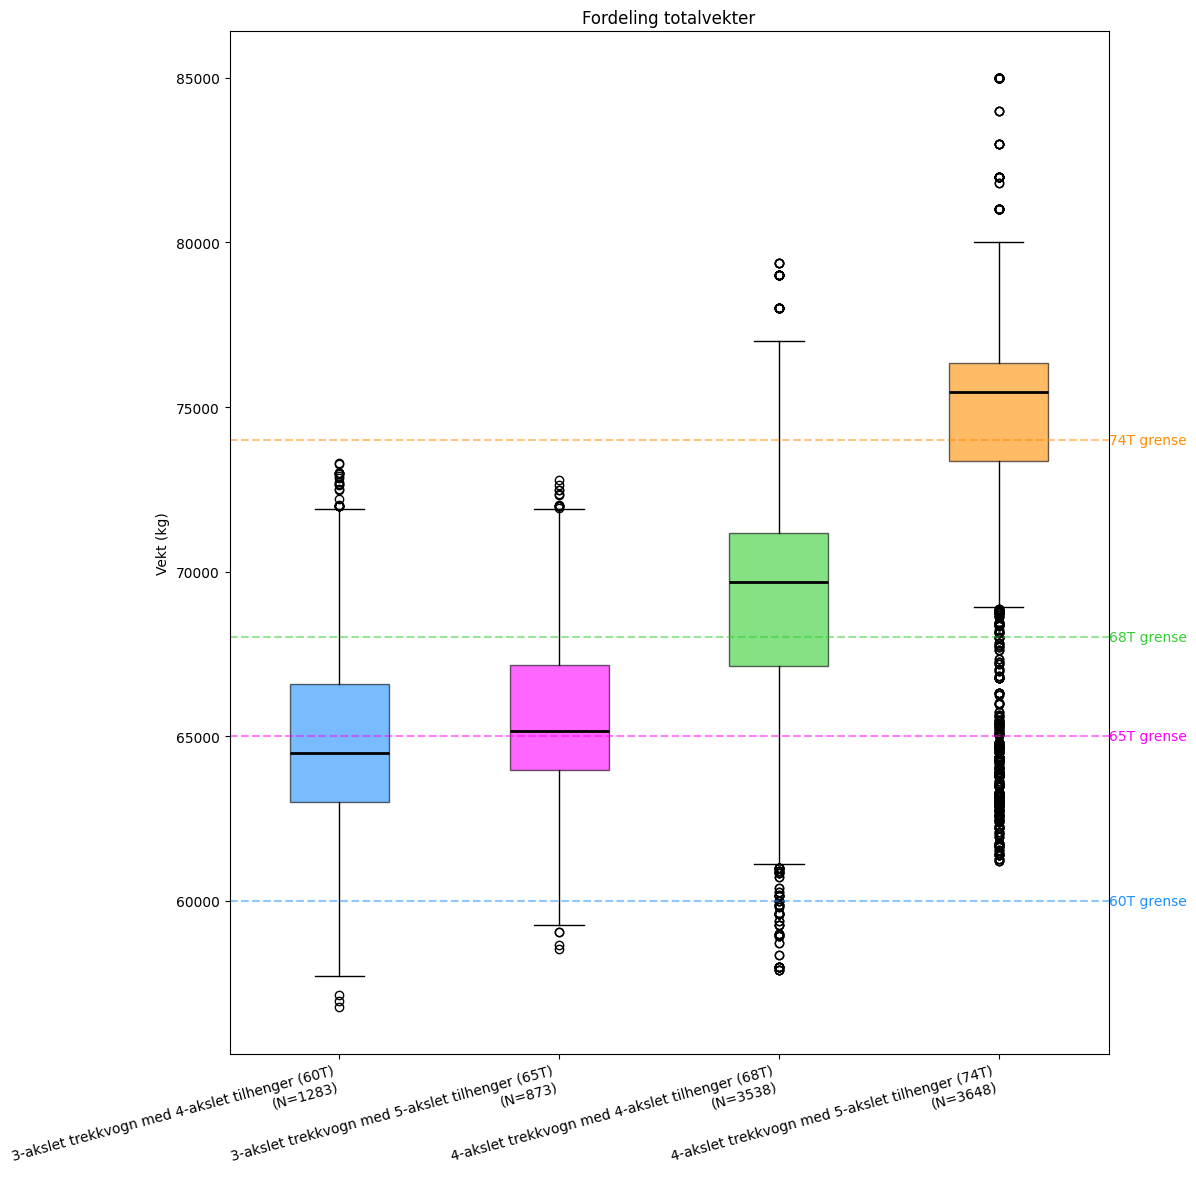
\includegraphics[width=0.75\textwidth]{images/boxplot_totalweights.png}
    \caption{Analyse av transportarbeid for ulike ekvipasjer}
    \label{fig:boxplot_totalweights}
\end{figure}